% !TeX spellcheck = en_GB
\usetikzlibrary{automata, positioning}

\section*{Mathematical Modelling: Using Markov chains to model bathroom queues}
\vspace{-.30cm}

\title{Mathematical Modelling: Using Markov chains to model chess games}

\begin{center}
	\textbf{Johnny Wong}\footnote{%
		Johnny Wong is a recent graduate of UNSW, Australia ({\tt johnny.c.wong@unswalumni.com})}
\end{center}

\vspace{5mm}

You come home from your morning run all sweaty and ready for a shower. As you approach the bathroom, you see the locked door and roll your eyes. Standing in your sweat soaked singlet, your little brother pokes his head out of his bedroom, chucks a deodorant at you before telling you he had already called dibs on the bathroom after you sister is finished. You throw the deodorant back at him and curse your house for having so few bathrooms.

Everyone has had to wait to use the bathroom at some point in their lives. It's common sense that the fewer bathrooms or more people there are, the longer you'd have to wait. But can we mathematically calculate how long we can expect to wait every day? One approach is with a technique called Markov chains.

For the rest of the article, let's consider the scenario where you have two bathroom between 4 people.

\subsection*{Markov chains}
To set up a Markov chain, you need several things: \textit{states} that represent the possible scenarios, \textit{probabilities} of moving from state to state throughout some measure of \textit{time}. We will unpack these 3 things in more detail below.

\subsubsection*{States}
A state is something that can describe the situation of interest at different points in time. If we are interested in the performance of a soccer team. We can have three states representing the outcome of a team's most recent game: Win, Lose, and Draw.

For our bathroom queueing problem, we are interested in how many people are using, or wanting to use, the bathroom at any point in time. So how many states do we need? Well with 4 people, there can be from 0 to 4 people wanting to use the bathroom, meaning we need 5 states. 

Let's label each state $0, \cdots, 5$, where state 0 means no one is wanting to use the bathroom. State 4 means four people want to use the bathroom, since there is only one bathroom available, this means 1 person is using it and there are 3 queuing up.

\subsubsection*{Time}
Time can be either discrete or continuous. The difference is best explained with an example or each.

\paragraph{Discrete time}
In the soccer team scenario, time wouldn't be measured in hours or days, each time point would be discrete and states can only change after each game. 

It is convention to start time at 0 and increment it by 1 as we reach the next discrete time point ($t=0, 1, 2, \cdots$) . We will represent the state at time $t$ as $X_t$.

If the team wins its first two games and loses the third, this sequence would be described as
$$ X_0 = \text{Win}, \, X_1 = \text{Win},\, X_2 = \text{Lose}$$

\paragraph{Continuous time}
We are all familiar with the concept of continuous time, it is how we perceive things everyday! Our Markov chain to model bathroom queues will use continuous time, because there is no obvious way to split real time into discrete chunks. 

In the previous example of the soccer game, states only change after each game. But people can leave or queue for the bathroom any point in time, meaning the states can change at any point in time.

\subsubsection*{Probability}
For Markov chains, we need to define the probabilities of moving from each state to every state (including itself). These probabilities are represented as a matrix. The numbers in this matrix represent different things, depending on whether we are working with discrete or continuous time.

A fundamental assumption of Markov chains is that the probability of moving from any state to the next is not impacted by any previous states, just the current one. This is called the \textbf{Markov property} and can be represented mathematically as:
$$ \Pr(X_{t+h}|\{X_s: s \leq t\}) = \Pr(X_{t+h}|X_t) \quad \text{for} \quad h > 0$$
If we take the current time to be $t$, the LHS of the above equation represents the probability of some future state given all previous states. The RHS represents the probability of the same future state but only given the current state, $t$. The fact that these probabilities are equal mean that any information about previous states has no impact on the direction of future states.


\paragraph{Discrete time probability matrix}
In discrete time, we need to describe the conditional probabilities of moving to every state given the current state. In other words, we need to define:
$$ \Pr(X_{t+1} = j|X_t = i) \quad \text{for all} \quad i, j$$
That is, the probability of moving to state $j$ given the current state is $i$. If $n$ is the number of states, then we need to provide $n^2$ probabilities. These are represented in the form of a $n\times n$ matrix, $P$ called the transition probability matrix.

Each column and row represent a state, and each element of the matrix is the conditional probability of moving from the state represented by the row, to the state represented by the column. Let's look at the example with the soccer team.

Suppose this soccer team is very streaky. If they won their last game, the probability of winning their next game is 80\%, and probability of losing their next game is 5\%. If they lost their last game, the probability of winning their next game is 30\%, and the probability of losing their next game is 60\%. And if they drew their last game, there is 25\% chance they win and 25\% chance they lose their next game.


\begin{figure}[h]
	\centering
		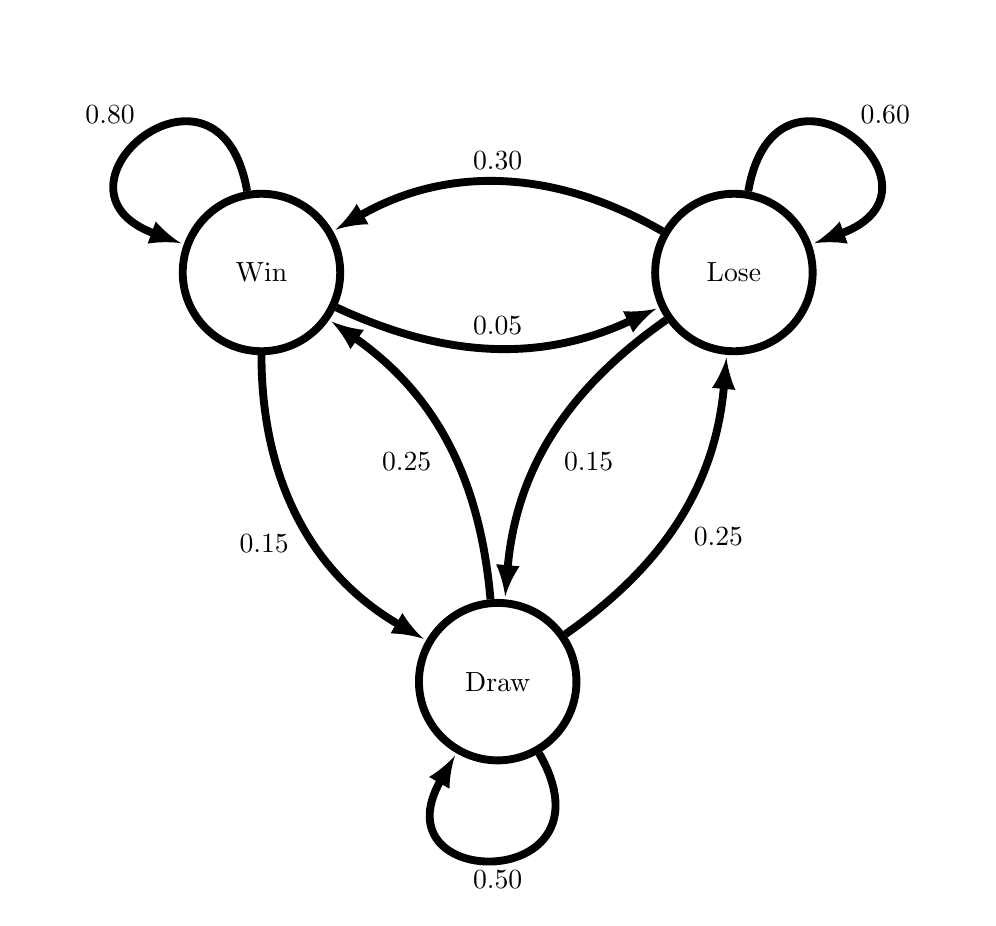
\begin{tikzpicture}
		% Node style
		\tikzset{node style/.style={state,
								minimum width=2cm,
								line width=1mm}}
							
		% Draw nodes
		\node[node style] at (0, 0) 		(W) {Win};
		\node[node style] at (6, 0) 		(L) {Lose};
		\node[node style] at (3, -5.196)	(D) {Draw};
		
		% Draw connectors
		\draw[every loop,
		auto=right,
		line width=1mm,
		>=latex
		]
		(W) edge[loop, out=100, in=160, 
				looseness=5] 				node {0.80} (W)
		(W) edge[bend right=25, auto=left] 	node {0.05} (L)
		(W) edge[bend right=30] 			node {0.15} (D)
		(L) edge[bend right=30] 			node {0.30} (W)
		(L) edge[loop, out=80, in=20, 
				looseness=5, auto=left]		node {0.60} (L)
		(L) edge[bend right=25, auto=left] 	node {0.15} (D)
		(D) edge[bend right=25, auto=left] 	node {0.25} (W)
		(D) edge[bend right=25] 			node {0.25} (L)
		(D) edge[loop, out=-60, in=-120, 
				looseness=5, auto=left]		node {0.50} (D);
		
	\end{tikzpicture}
	\caption{Visual representation of the soccer team's probabilities}
	\label{fig: soccer team visual}
\end{figure}

Figure \ref{fig: soccer team visual} is a visual way of representing the above information, and is easier to digest. Figure \ref{fig: soccer team transition matrix} shows the probability transition matrix and is even more compact.

\begin{figure}[H]
	\centering
	
$$P=\bordermatrix{\text{State} 	&\text{Win} &\text{Lose}& \text{Draw}\cr
			 	\text{Win} 	&   0.80  	&	0.05	&	0.15	\cr
		 	 	\text{Lose}	& 	0.30  	&	0.60	&	0.10	\cr
	 	 		\text{Draw}	&	0.25	&	0.25	&	0.50	}$$
 	 \caption{Transition probability matrix representing the soccer team's probabilities.}
 	 \label{fig: soccer team transition matrix}
\end{figure}

The rows and columns have been labelled to easily see what each number means. The element in the second row (Lose) first column (Win) is $0.30$, meaning there is a 30\% chance of winning the next game if the team had lost its last game.
\\

There are a few things to check when creating a probability transition matrix.
\begin{itemize}
	\item All entries are between 0 and 1 inclusive.\\
	This is needed as each entry represents a probability
	\item The sum of all rows is 1.\\
	This ensure that the system can only transition between the defined states. The sum of the first row in figure \ref{fig: soccer team transition matrix} represents the probability that, given the team won its last game, it will either win, lose, or draw the next game. This is necessarily 1 as it includes all possible outcomes.
\end{itemize}
You can verify that both these conditions are satisfied in the above case.

\subsubsection*{Limitations of the model}
Now that there is a numeric answer to our question, it is important to look back on the process and acknowledge the limitations of our method.

One of the main assumptions of Markov chains is the Markov property. This is also referred to as \textit{memoryless} andstates that it doesn't matter what's happened in the past, the behaviour of the system only depends on what the current state is. We've assumed that the expected time spent in the bathroom is 5 minutes. So as soon as someone walks in, it is expected they'll leave after 5 minutes. Under the Markov property, if someone has been in the bathroom for 10 minutes already, is is still expected that they will leave after another 5 minutes.

Similarly, the rate at which someone goes to the bathroom stays the same regardless of if they've gone 10 times already today or haven't gone at all.
\\

While these assumptions may seem unrealistic at first, it isn't that unreasonable when you look at it's implications in aggregate. Markov chains, through their memorylessness, implicitly assume that the number of bathroom visits is Poisson distributed, and the time spend in the bathroom is Exponentially distributed. 